\section{Fourier Transformation}
Our goal is to decrease the intensity of the spyders and speckles in the data. In our data from HD142527 the main disturbing effects are the spyders. With the transformation to the $r$-$\varphi$ plane the spyders now are parallel to the $r$-axis. When comparing different data sets from the same observation we find that the spyders change there position, but the distance between them stays the same. It is a periodic pattern. This brings up the idea, if the spyders are represented by a set of frequencies in the frequency plane. If this is the case, the suppressing of some of the frequencies in the frequency plane would result in a suppressing of the spyders in the image plane. The advantage of this method would be that it could be applied to the complete data set and one can ignore the fact that the spyders wander along the $\varphi$-axis. Also we should be able to suppress the spyders without destroying the information below them.\\
In the following we are going to investigate the properties of a fourier transformation and the effect of suppressing certain frequencies on the image plane.\\

\subsection{Fourier Transformation of Lines and Beams}
We first want to investigate the effect of some simple signals in the image plane on the frequency plane. We choose these signals similar to the shape of the spyders or to the shape of a potential exoplanet, with the goal to identify similar characteristics in the frequency plane of the data.\\
Firstly, the we transform a single line (has the width of one pixel) in vertical or horizontal direction to the fourier plane. A single line in vertical direction ($y$-axis) means that we have a constant signal along the $y$-axis, but we have one in $x$ direction, namely a one pixel wide peak at the $x$ position of the line. So we expect that all $y$-axis frequencies in the fourier transformed image to be zero, this means that only at $y$ frequency zero we have non-zero values which describe the periodicity in $x$ direction.\\
As we can see from figure \ref{fig:fft_line} the transformation of a single line results into a single line in the frequency plane. The line in the frequency plane is perpendicular to the line in the image plane and is located in the center. This confirms our expectations. 
\begin{figure}[H]
	\centering
		\subfigure[]{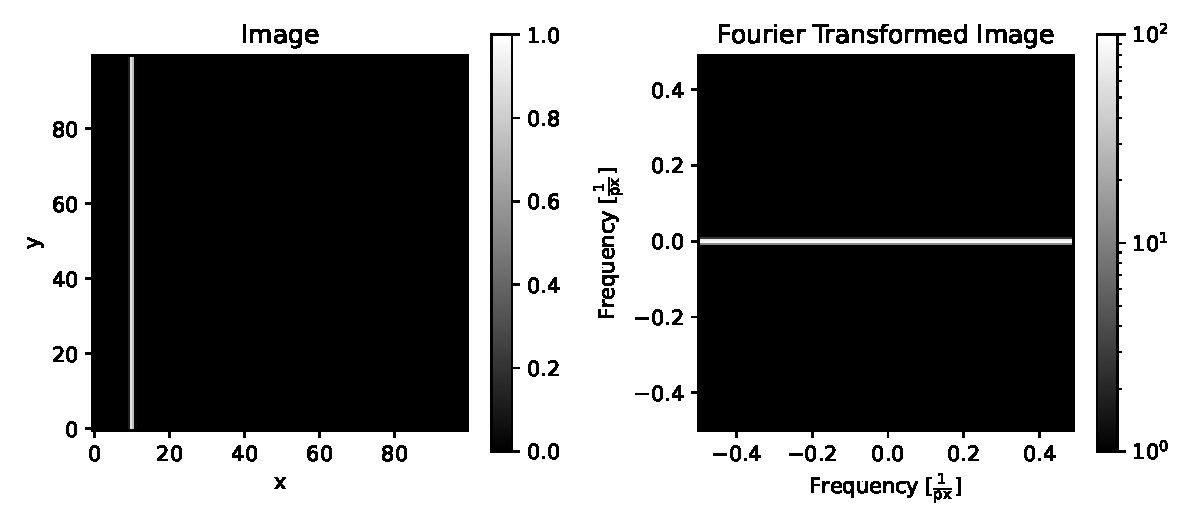
\includegraphics[width=1.0\textwidth]{pics/fft_simulationoneline.pdf}}
		\subfigure[]{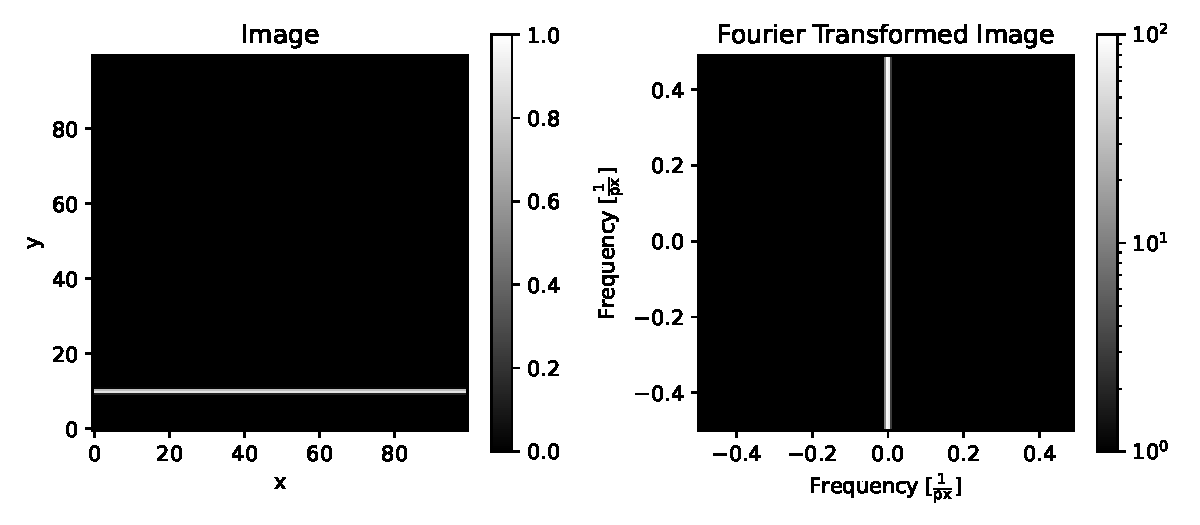
\includegraphics[width=1.0\textwidth]{pics/fft_simulationoneline_horizontal.pdf}}
\caption{The image of a vertical line (a) and of a horizontal line (b) (images on the left side) are transformed to the frequency plane (images on the right side).}
\label{fig:fft_line}
\end{figure}
To explore the frequency plane further we plot the intensity at the $y$ equals zero along the $x$-axis (frequency plane of image shown in figure \ref{fig:fft_line} (a)). This describes the periodicity of the image in horizontal direction. As we see in figure \ref{fig:fft_line_cut} the intensity is almost constant, with a periodicity of $0.1 \frac{1}{\mathrm{px}}$. We conclude that if we have a single line at position $x_{\mathrm{line}}$ in the image plane we get a periodic signal in the fourier plane where the wave length is given by $\frac{1}{x_{\mathrm{line}}}$. However, the amplitude of this signal is really small, since it is only one single line.  
\begin{figure}[H]
	\centering
		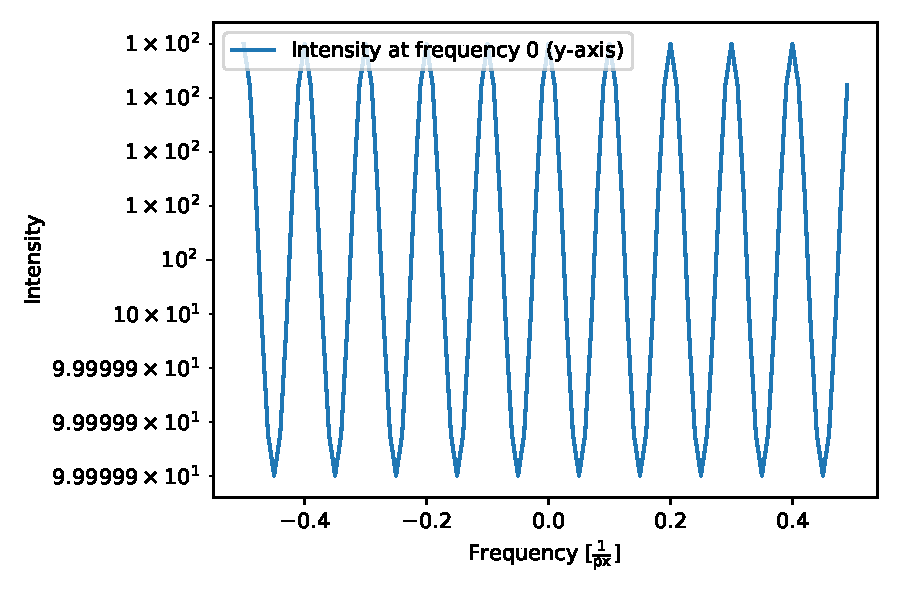
\includegraphics[width=0.8\textwidth]{pics/fft_simulation_cutoneline.pdf}
		\caption{The intensity of the fourier transformed image in figure \ref{fig:fft_line} (a) at y frequency zero.}
		\label{fig:fft_line_cut}
\end{figure}
As a next step we want to find out what happens, if we insert a periodic signal into the image plane in the form of equally spaced lines? Figure \ref{fig:fft_lines} shows an image where there are several vertical lines with a spacing of 20 pixels. As in the case of the single line the image is constant in $y$ direction and so all vertical frequencies are assigned zero. In $x$ direction the lines create a periodic signal with frequency $\frac{1}{20} = 0.05 \frac{1}{\mathrm{px}}$. On the right side of \ref{fig:fft_lines} we see the fourier transformation of the image with the equally spaced lines and \ref{fig:fft_lines_cut} shows a horizontal cut through the center. 
\begin{figure}[H]
	\centering
		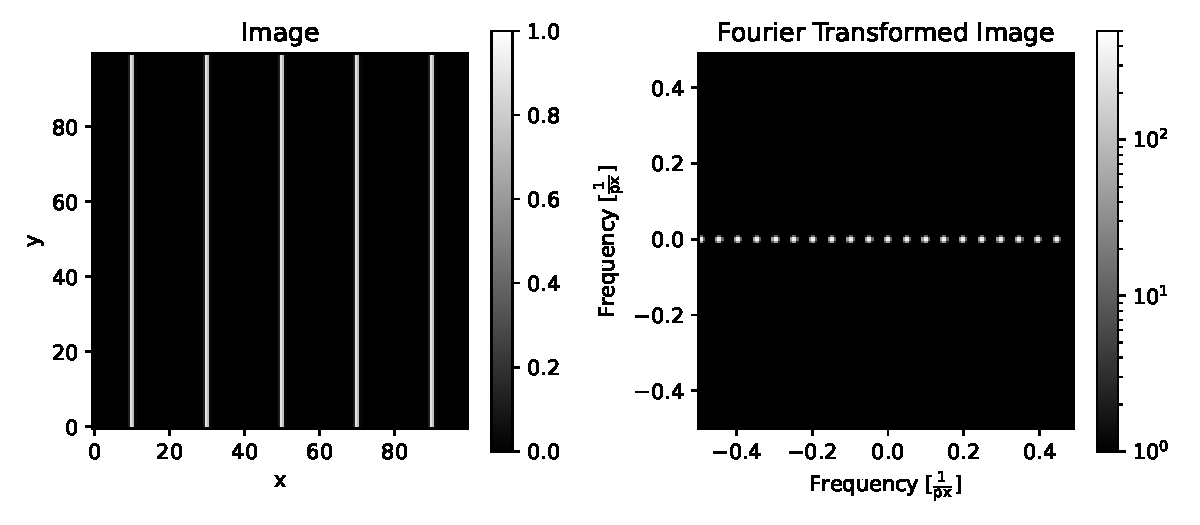
\includegraphics[width=1.0\textwidth]{pics/fft_simulationmorelines.pdf}
		\caption{The image with several equally spaced one pixel thick lines on the left is transformed to the frequency plane, see image on the right.}
		\label{fig:fft_lines}
\end{figure}
\begin{figure}[H]
	\centering
		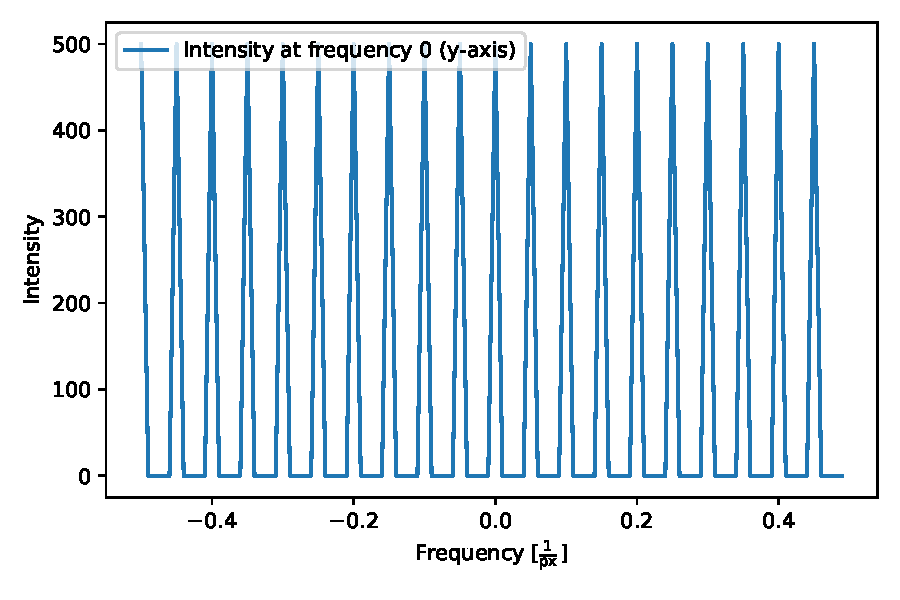
\includegraphics[width=0.8\textwidth]{pics/fft_simulation_cutmorelines.pdf}
		\caption{The intensity of the fourier transformed image in figure \ref{fig:fft_lines} at y frequency zero.}
		\label{fig:fft_lines_cut}
\end{figure}

In the appendix we show, what happens if one line is missing -> not completely periodic.